\documentclass[]{report}

\usepackage[portuguese]{babel}
\usepackage[utf8]{inputenc}
\usepackage{graphicx}
\usepackage{hyperref}
\usepackage{mdwlist}
\usepackage{pslatex}
\usepackage{makeidx}
\usepackage{textcomp}
\usepackage{float}
\usepackage{amsmath}
\setlength{\oddsidemargin}{0pt}
\setlength{\evensidemargin}{0pt}
\setlength{\textwidth}{15cm}

% Title Page
\title{}

\makeindex
\begin{document}
\begin{titlepage}
\begin{center}

\textsc{\LARGE Universidade Federal de Santa Maria}\\[1.5cm]
\textsc{\Large Centro de Tecnologia}\\[0.5cm]
\textsc{\Large Departamento de Eletrônica e Computação}\\[0.5cm]
\textsc{\Large Disciplina: Princípios de Telecomunicações}\\[0.5cm]
\setlength{\oddsidemargin}{0pt} % Tirar as margens gigantes que o LaTeX põe
\setlength{\evensidemargin}{0pt} % evitar desperdício de papel
\setlength{\textwidth}{15cm}
\end{center}

\vspace*{5cm}
\begin{center}
{\huge \bfseries Estudo sobre Modulação de Sinais}\\[0.4cm]
\end{center}

\vspace*{130px}
\begin{flushright}
\emph{Autores:}
Caio S. Guedes $<$\url{caio_ee@hotmail.com}$>$ \newline
Marcelo Brum $<$\url{marcelobrum.rs@gmail.com}$>$ \newline
Renan Pinheiro $<$\url{renan.ee.ufsm@gmail.com}$>$. \newline



\end{flushright}
\begin{center}
Santa Maria, \today.

\end{center}


\end{titlepage}
\tableofcontents

\chapter{Introdução}

Em telecomunicações, modulação é a modificação de uma onda eletromagnética, para que informação seja transportada por meio de uma onda portadora. Normalmente seu objetivo é facilitar a comunicação através da redução do tamanho das antenas de receptor e transmissor.

Neste trabalho serão abordadas as práticas feitas em laboratório, na discplina de Princípios de Telecomunicações, visando estudar o funcionamento das modulações em amplitude (AM) e em frequência (FM). Também será abordada a modulação por códigos de pulso (PCM). 

\chapter{Experimento 1: Modulação AM a diodo}
\section{Fundamentação Teórica}
Para ambas as modulações, sejam:

\begin{itemize}
\item um sinal senoidal modulante dado por 

\begin{equation}\label{eq_modulante}
v_s = A_s \cos(\omega_s t + \phi)
\end{equation}

\item uma portadora dada por

\begin{equation}\label{eq_portadora}
v_c = A_c \cos(\omega_c t + \phi)
\end{equation}
\end{itemize}
tal que $\omega_c > \omega_s$. A fase dos sinais é fixa em $0$, assim eliminando-se $\phi$. 

\subsection{Modulação em Amplitude com Portadora Suprimida (AM-DSB-SC)}
Nos domínios do tempo e da frequência ela é dada por

\begin{equation}\label{eq_am_dsb_sc_tempo}
v_m = v_s v_c = A_s A_c \cos(\omega_s t) \cos(\omega_c t)
\end{equation}

o que no domínio da frequência dá
\begin{equation}
\mathcal{F}(V_m)= \frac{A_s A_c \delta(\omega_s - \omega_c) + \delta(\omega_s + \omega_c)}{2}
\end{equation}

representado no gráfico
\begin{figure}[H]
\begin{center}
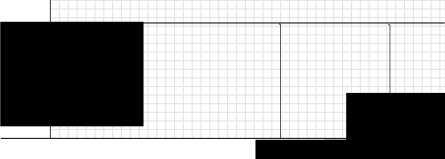
\includegraphics[scale=0.8,clip]{./imagens/frequencia_AM_DSB_SC}
\end{center}
\caption{O sinal AM-DSB-SC no domínio da frequência.}
\label{fig:am_dsb_sc_frequencia}
\end{figure}

O principal problema dessa modulação é que o receptor precisa gerar sua própria portadora para demodulação do sinal. Se ela não estiver sintonizada na exata frequência da portadora original, tem-se a distorção do sinal demodulado. 

\subsection{Modulação em Amplitude com Portadora (AM-DSB)}
Nesta modulação, transmite-se a portadora juntamente ao sinal, simplificando a demodulação. Então a modulação pode ser escrita como
\begin{equation}\label{eq_am_dsb_tempo}
v_m = \underbrace{v_s v_c}_{AM-DSB-SC} + \underbrace{v_c}_{portadora\ adicional} = v_c [1 + v_s]
\end{equation}

e assim no domínio da frequência tem-se que o espectro deste sinal é dado por

\begin{equation}
\mathcal{F}(V_m)= \frac{A_s A_c \delta(\omega_s - \omega_c) + \delta(\omega_s + \omega_c) + A_c \delta(\omega_c)}{2}
\end{equation}

Dessa forma, perde-se eficiência mas a demodulação se torna mais simples, como será visto no decorrer deste capítulo.

\section{Procedimento experimental}

Problema proposto:
\begin{quote}
Implemente o circuito da Figura 1 e calcule a frequência de ressonância do filtro passa faixa. Ajuste a frequência de $E_o(t)$ para o valor calculado. Ajuste a frequência de $a(t)$ para 1KHz. Faça a amplitude de $E_0(t)$ igual a 10V pico a pico e a de $a(t)$ 3V pico a pico. Apresente suas conclusões a respeito do uso do filtro e da frequência de ressonância obtida.
\end{quote}


O circuito da figura \ref{fig:demodulador_AM_diodo} foi montado em uma \textit{protoboard}:
\begin{figure}[H]
\begin{center}
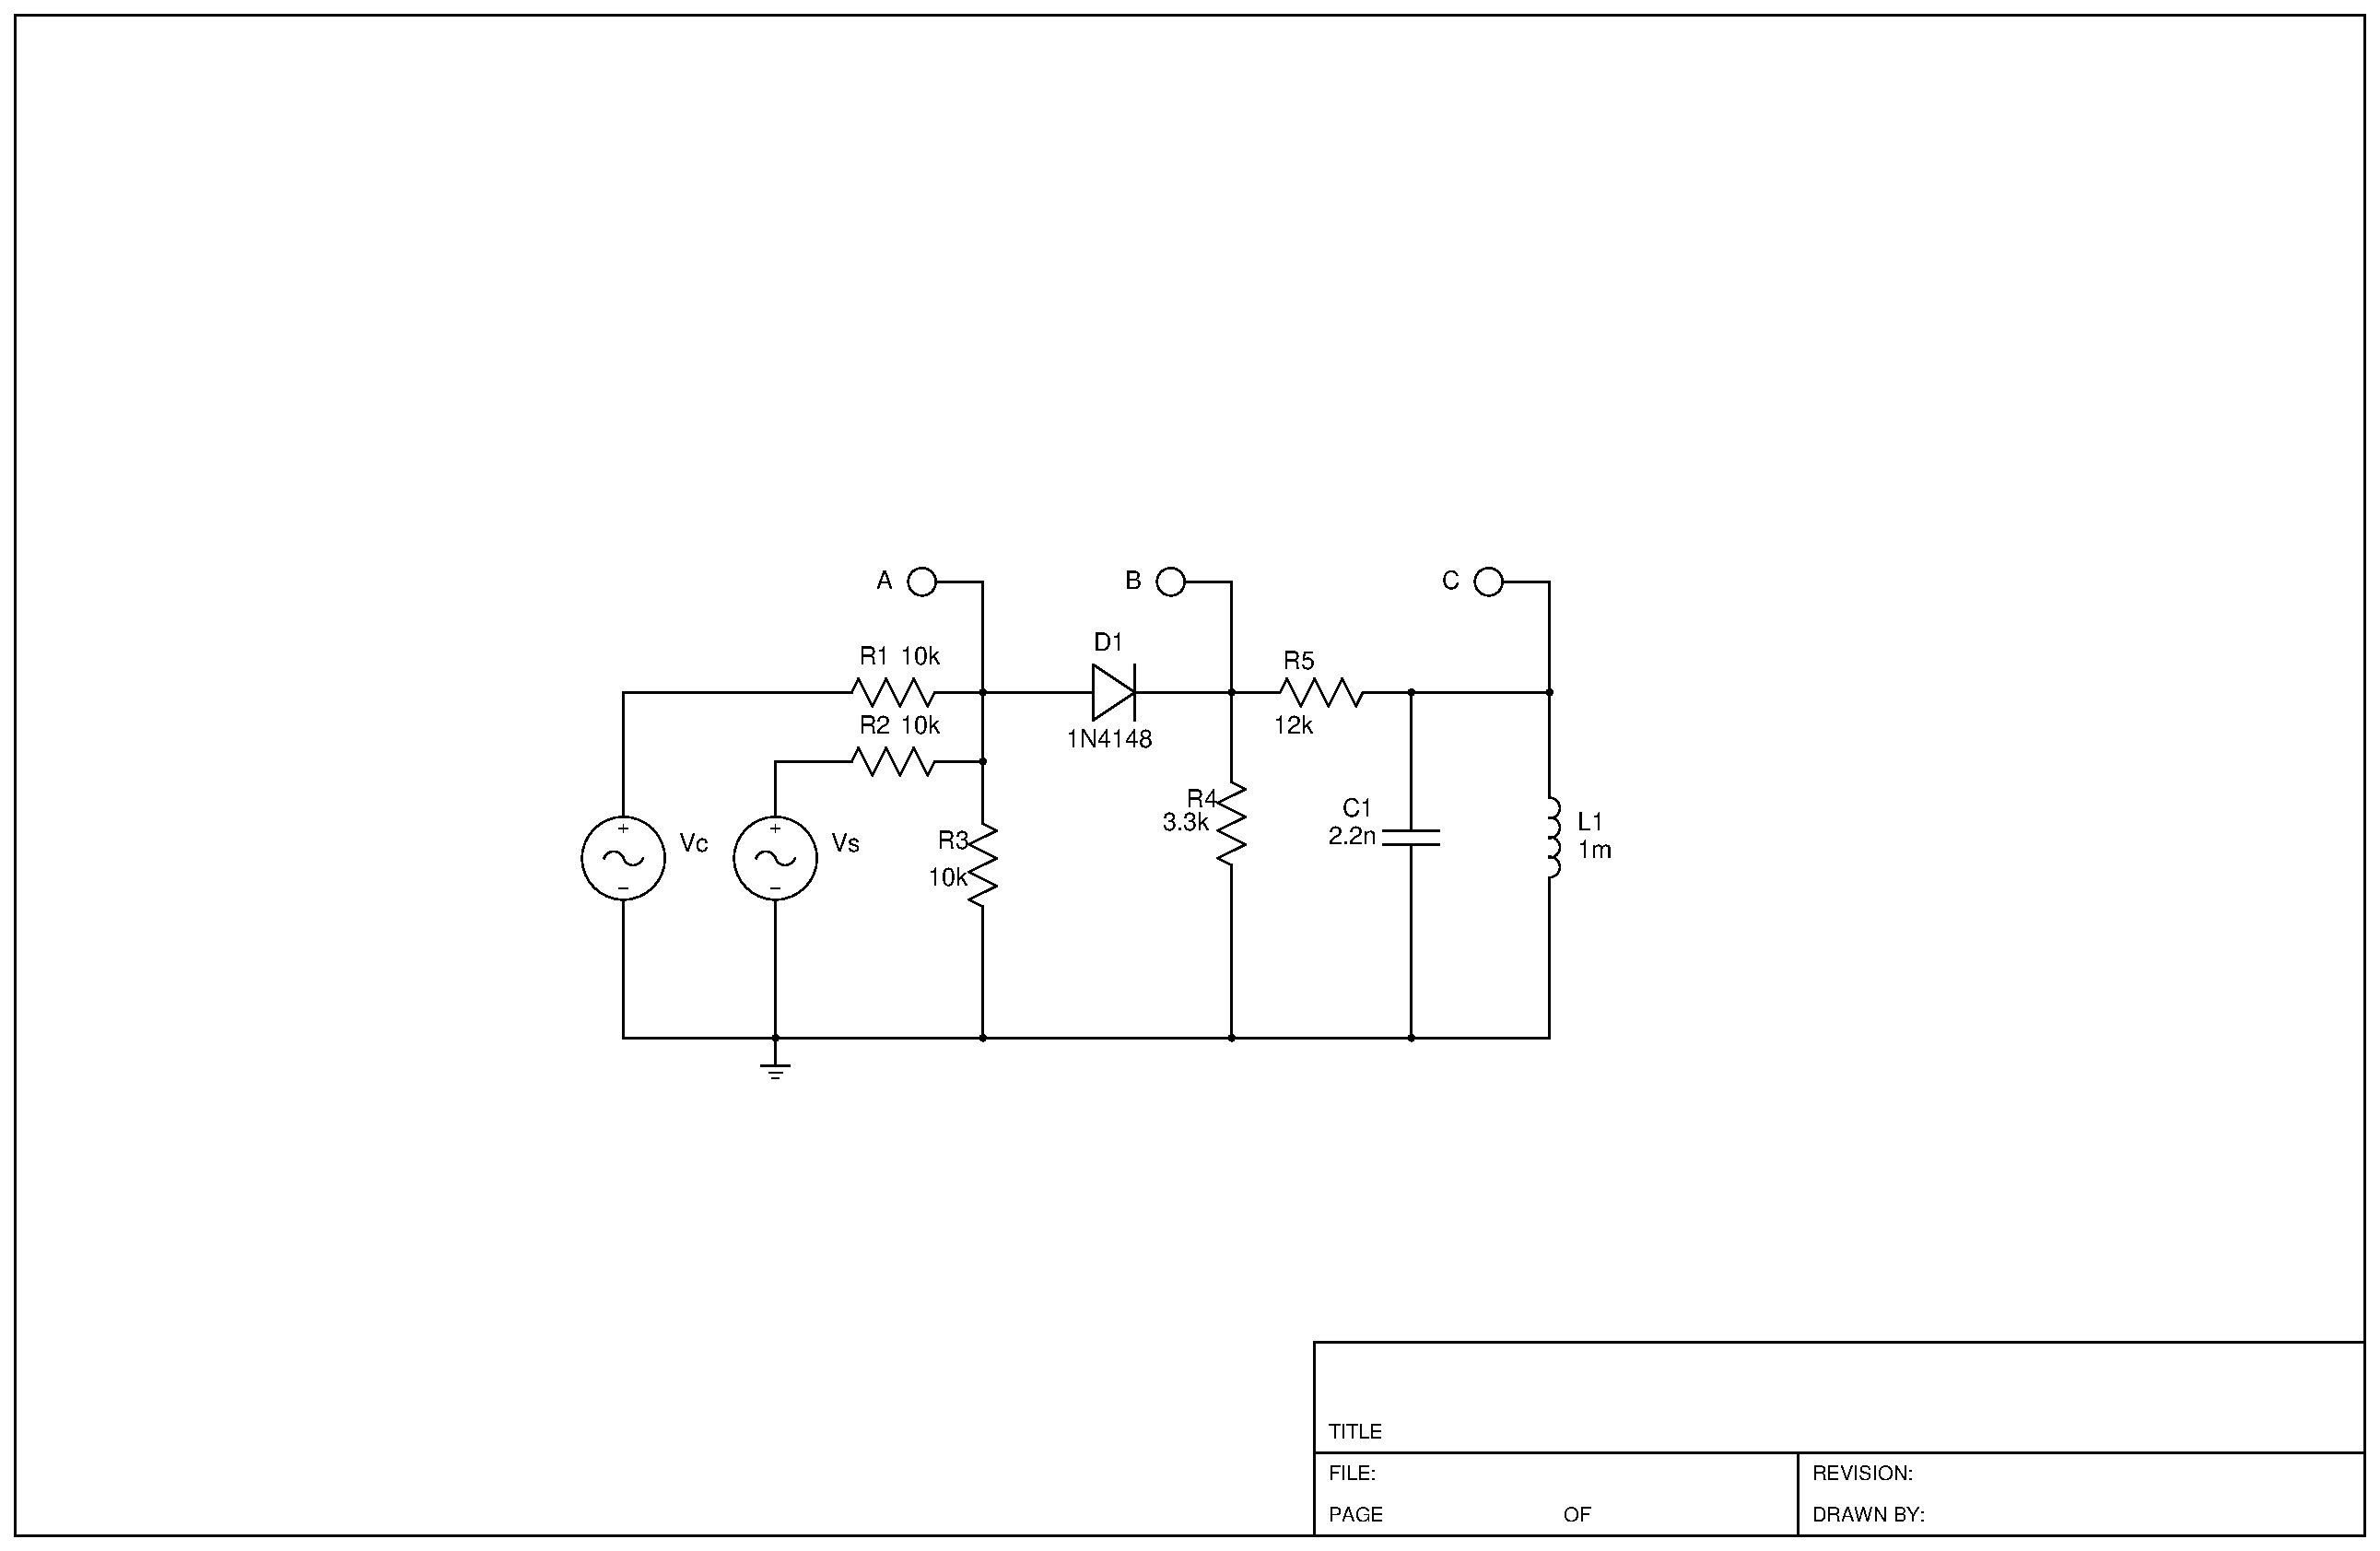
\includegraphics[scale=0.4,clip]{./imagens/AM_Modulator_Diode}
\end{center}
\caption{Modulador AM a diodo.}
\label{fig:demodulador_AM_diodo}
\end{figure}

Para sintonizar a portadora, calcula-se a frequência de ressonância do filtro LC da saída:

\begin{equation}
f_0 = \frac{1}{2 \pi \sqrt{LC}}
\end{equation}

Para os valores fornecidos ($C = 2,2 nF$ e $L = 1000 \mu F$) ter-se-á que essa frequência será de cerca de 107 KHz. 

Após sintonizados os sinais de portadora e da modulante, na saída (ponto C) constata-se a modulação do sinal. Neste contexto, o indutor e o capacitor agem no sentido de limitar a faixa de frequência do sinal modulado.

Disto se determinam:
\begin{itemize}
\item{\bf Frequências dos sinais portador e modulante:} 107 KHz e 1 KHz, respectivamente.

\item{\bf Forma de onda:}
\begin{figure}[H]
\begin{center}
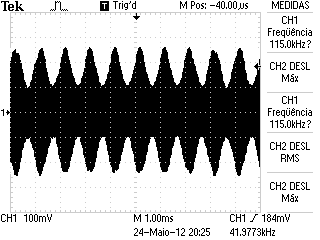
\includegraphics[scale=0.65]{./imagens/AM_Dominio_Tempo}
\end{center}
\caption{Sinal à saída do modulador (ponto \textit{C} no esquemático).}
\label{fig:onda_AM}
\end{figure}
\begin{figure}[H]
\begin{center}
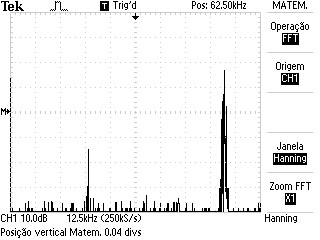
\includegraphics[scale=0.65]{./imagens/AM_Dominio_Frequencia}
\end{center}
\caption{Espectro de frequência deste sinal.}
\label{fig:frequencia_AM}
\end{figure}

Pelo espectro verifica-se que a modulação é do tipo \textbf{AM-DSB}.
\item{\bf Índice de modulação:}
O índice de modulação ($IM$), para um sinal puramente senoidal, é calculado por

\begin{equation}\label{indice_modulacao}
I_m = \frac{M_{max} - M_{min}}{M_{max} + M_{min}}
\end{equation}

Do gráfico \ref{fig:onda_AM} mede-se aproximadamente $M_{min}$ = 100 $mV$ e $M_{max}$ = 240 $mV$; colocando-se esses valores na equação \ref{indice_modulacao} tem-se que $I_m \approx 41,17 \%$.
\item{\bf Potência média do sinal:}

A potência média do sinal, assumido que ele esteja ligado à uma carga de 1 $\Omega$, pode ser calculada por

\begin{equation}
P = \frac{{V_m}^2}{R} = \frac{1}{T}\int\limits_{0}^{T}{V_m^2}dt
\end{equation}

Pode-se demonstrar que no nosso caso isso resulta em

\begin{equation}
P = \frac{{V_p}^2}{2}
\end{equation}

Considerando as bandas laterais teremos que

\begin{equation}
P_t = \frac{{E_p}^2}{2} + \frac{{I_m}^2 {E_p}^2}{4}
\end{equation}

Assim, determina-se que para o nosso caso a potência média (para o caso teórico de conexão à carga de 1 $\Omega$) será de aproximadamente 54 W.


\end{itemize}
\subsection{Modulação por diodo}
Pergunta: \begin{flushright}
\textit{Explique como o diodo possibilita a modulação do sinal Eo (t) no circuito implementado na matriz de contatos e apresente o equacionamento que demonstra tal método de modulação.}
\end{flushright}

Suponhamos o diodo como uma chave que permite apenas a passagem da região positiva da onda da portadora. Esse diodo pode ser considerado como um dispositivo não linear, expresso por $e_1(t) = a e_0(t) + b e^2_0(t)$. 

Ao diodo chega a soma dos sinais da portadora e da modulante: $e_0(t) = v_s + v_c$.

\subsection{Demodulação do sinal}

\chapter{Experimento 2: Modulação AM a transistor}

\begin{figure}[H]
\begin{center}
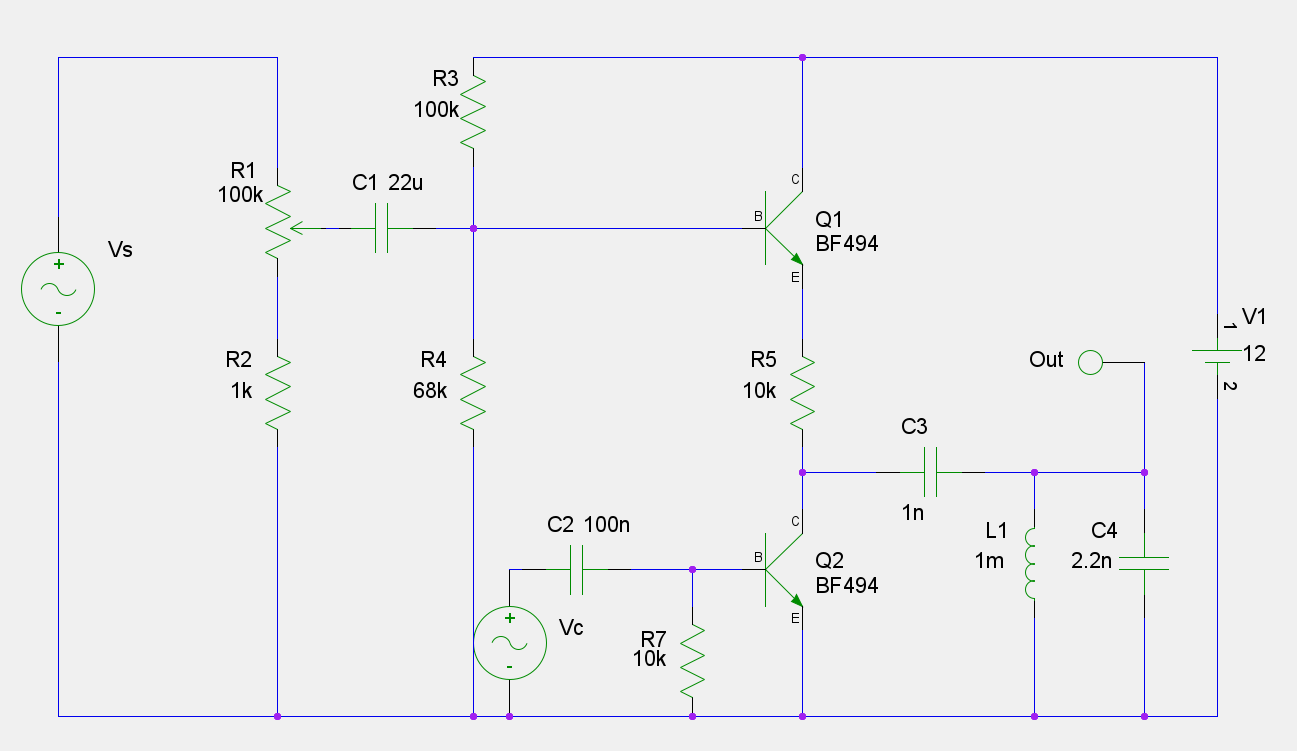
\includegraphics[scale=0.25,clip]{./imagens/AM_Modulator_Transistor.png}
\end{center}
\caption{Modulador AM a transistor.}
\label{fig:modulador_AM_transistor}
\end{figure}

O sinal modulado é gerado utilizando-se os transistores BF494 \cite{BF494}, de alta frequência (até 120 MHz, conforme sua \textit{datasheet}). O sinal de áudio oscila pelo transistor $Q_1$, e a portadora pelo transistor $Q_2$. Tal circuito age como um multiplicador para os sinais. A junção desses sinais é feita no capacitor $C_3$, que já remove o nível DC que existe na saída dos transistores como consequência da polarização, e o filtro LC formado por $L_1$ e $C_4$ tratará de permitir apenas o sinal de frequência desejada.

\chapter{Experimento 3: Transmissão e recepção de FM; modulação em fase}
\section{Fundamentação teórica}
\section{Modulação FM}
\section{Modulação em fase}

Seja uma portadora dada por
\begin{equation}\label{portadora_PM}
v_p = A_p \sin(\omega_p t + \phi_p).
\end{equation}

e uma modulante dada por uma função $v_s$ qualquer. Assim teremos que o sinal modulado ficará
\begin{equation}\label{modulada_PM}
v_m = A_p \sin(\omega_p t + v_s + \phi_p)
\end{equation}

No receptor haverá um circuito que medirá essa variação de fase, decodificando-na em um sinal.

A modulação de fase (PM – \textit{phase modulation}) não é amplamente utilizada em transmissões de rádio, devido principalmente a tendência desse tipo de modulação necessitar de um equipamento mais complexo no recebimento do sinal, e também pela possibilidade de ocorrerem alguns problemas de ambiguidade na mudança do sinal (por exemplo, uma mudança de +180° ou -180° seria a mesma).

Para a modulação em fase, temos uma mudança na fase da portadora.

\section{Demodulação de FM}
A demodulação deste tipo de sinal é muito mais complexa do que a demodulação feita para os sinais em amplitude modulada. As principais estratégias para a demodulação são:
\subsection{Detector de Quadratura}
O detector de quadratura divide o sinal modulado em dois. Um os sinais passa através de um capacitor de alta reatância, assim deslocando a fase do sinal em 90 graus. Esse sinal é aplicado então a um circuito LC, cuja frequência natural de ressonância é a mesma da portadora. Se a frequência do sinal modulado em frequência for igual à da portadora, os dois sinais então terão um defasamento de 90 graus entre eles, ou seja, estarão em \textit{quadratura de fase}.

Os dois sinais são então multiplicados juntos em um dispositivo analógico ou digital que funciona como um detector de fase, isto é, um dispositivo o qual sua saída é proporcional a diferença de fase dos dois sinais.
No caso de um sinal recebido que não tenha sido modulado, a saída do detector de fase será, em média, zero. No caso de um sinal modulado, então haverá uma diferença na frequência deste sinal em relação a frequência central (frequência da portadora), neste caso o circuito LC ressonante vai deslocar a fase do sinal recebido do capacitor, sendo assim a variação total da fase do sinal serão os 90 graus impostos pelo defasamento do capacitor e mais uma variação (positiva ou negativa) imposta pelo circuito LC. A saída do detector de fase agora difere de zero, e dessa forma o sinal original usado para modular a onda da portadora pode ser recuperado.
\subsection{\textit{Phase-locked Loop} (PLL)}
O laço de bloqueio de fase não necessita de um circuito LC ressonante para realizar a demodulação. Ele é composto de um bloco detector ou comparador de fase, um filtropassa-baixa e um VCO(voltage controlled oscillator). Neste sistema, o oscilador controlado por tensão tem sua fase bloqueada por um laço de realimentação negativa, forçando o VCO a seguir as variações do sinal modulado de entrada. A tensão resultante de baixa frequência que sai do filtro passa-baixa e faz com que o VCO siga a frequência do sinal de entrada é o sinal demodulado.
\subsection{Detector de Foster-Seeley}
Este circuito foi criado em 1936 por Dudley E. Foster e Stuart William Seeley visando a construção de um controle de freqüência automática de receptores, porém encontrou utilidade também como demodulador de freqüência. 
Ele utiliza um transformador de radiofreqüência que converte variações em freqüência para variações em amplitude. O transformador, sintonizado na freqüência da portadora, é ligado a dois diodos retificadores, semelhante a um retificador de onda completa em ponte.
Se a freqüência de entrada for a mesma da portadora, as duas metades do circuito do transformador de radiofreqüência produzem a mesma queda de tensão e a saída é igual a zero. A medida que ocorrem diferenças o equilíbrio entre as duas metades do secundário do transformador varia e o resultado vem a ser uma tensão proporcional ao desvio de frequência da portadora.
Note que esse circuito é sensível a variações na amplitudade, diferente de alguns detectores. Isso implica na necessidade do uso de uma etapa com um amplificador limitador antes do detector, removendo assim as variações indesejadas na amplitudade as quais seriam adicionadas como ruídos.

\chapter{Experimento 4: Modulação por código de pulso (PCM)}
\section{Introdução}
PCM é uma técnica para a representação de sinais analógicos convertidos para formato digital, visando transmissão ou posterior processamento. Uma codificação em PCM transforma uma amostra quantizada em um número codificado. \cite{renatodatacom}

Fundamentalmente, a técnica consiste na quantização dos dados através de um conversor A/D. No lado do receptor existirá um conversor D/A que irá fazer o processo oposto.

\chapter{Conclusão}
Modulações analógicas, como as vistas neste trabalho, continuam sendo importantes devido à sua simplicidade e baixo custo de implementação. 

\bibliographystyle{alpha}
\begin{thebibliography}{100}
\bibitem{renatodatacom}
 MACHADO, R. 
 \textbf{Notas de aula da disciplina de Comunicação de Dados.}
 Disponível em \url{http://www.ufsm.br/gpscom/professores/Renato\%20Machado/comunicacaodedados.html}. Acessado em 12/06/2012.
 
\bibitem{lamar}
LAMAR, V. M. \textbf{Modulação em Amplitude}. Disponível em \url{http://www.cic.unb.br/~lamar/te060/Apostila/Capitulo2.pdf}. Acesso em 23/06/2012.

 
\bibitem{BF494}
\textbf{BF494, BF495 NPN Medium-Frequency Transistors}. Disponível em \url{http://www.datasheetcatalog.org/datasheet/philips/BF494B.pdf}. Acesso em 23/06/2012.

\bibitem{teleco}
\textbf{O Início da Digitalização - Telefonia Fixa}. Disponível em \url{http://www.teleco.com.br/tutoriais/tutorialciclos/pagina_4.asp}. Acesso em 27/06/2012.

\bibitem{campos}
\textbf{Modulação e Demodulação de Sinal}. Disponível em \url{http://www.del.ufms.br/PCI_T1/G6/Modulacao.htm}. Acesso em 28/06/2012.
\end{thebibliography}
\end{document}          
